% !TEX root = Thesis.tex
\chapter{Layout Migration Flow}\label{chap:migration}

  In this section, we introduce the overall flow of the proposed layout migration methodology.
  Generally, analog design follows hierarchical design concept that produces structural design. 
  Hence, to extend the idea, we also consider the multilevel analog design in our prototyping framework.Fig.~\ref{fig:Flow} shows the overall flow diagram.
  The flow is mainly separated into 3 stages: 1) the layout extraction and preservation stage, 2) the layout prototyping stage and 3) the wire segment refinement. 
  
  
  \begin{figure}[ht]
  \centering
  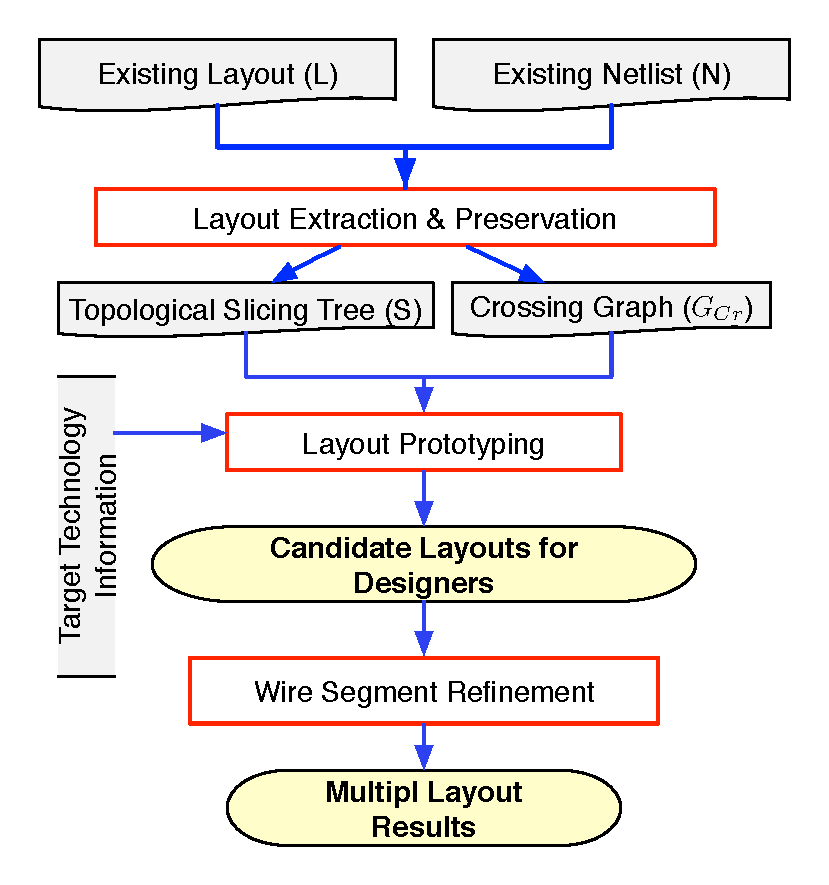
\includegraphics[width=0.5\textwidth]{Fig/Flow.eps}
  \caption{Overall flow of the proposed layout migration scheme.} 
  \label{fig:Flow}
  \end{figure}

  \begin{table}
    \begin{center}
    \caption{Comparison on Analog Layout Migration Approaches}\label{table:MigrateComp}
    \scriptsize
    %\begin{tabular}{|m{2cm}|m{2cm}|m{2cm}|m{2cm}|m{2cm}|}
    \begin{tabular}{|c|c|c|c|c|}
      \hline
      & \cite{msc-bhattacharya-tcad06} & \cite{ALP_YPWeng_iccad2011} & \cite{Chin_DMR_ICCAD2013} & Our Approach \\
      \hline
      Layout Constraints & Preserved & Preserved & Preserved & Preserved \\
      \hline
      Placement topology  & Keep origin & Multi-prototypes & Already given & Multi-prototypes \\
      \hline  
      Routing behavior  & Partially preserved &  Manually completed &  Preserved routing & Preserved routing \\
      \hline
      \#Migrated Layout &  1 &  Multi-Solutions & Multi-Solutions & Wires refined Multi-Solutions \\
      \hline
      Sign-off Time &   slow &  slow &  fast &  fast \\
      \hline
    \end{tabular}
    \end{center}
  \end{table}

  In comparison with current migration mechanisms, Table~\ref{table:MigrateComp} shows the different criterion to examine the disparity. There are 3 current migration styles, \cite{msc-bhattacharya-tcad06}, \cite{ALP_YPWeng_iccad2011} and \cite{Chin_DMR_ICCAD2013}, mentioned in Table~\ref{table:MigrateComp}. For analog layout constraints, each approach is able to preserve specific constraints such as symmetry constraints and matching constraints. For placement topology, \cite{msc-bhattacharya-tcad06} aims to keep the exactly same topology as the existing layout, \cite{ALP_YPWeng_iccad2011} successfully produces multiple placement candidates and the placement in \cite{Chin_DMR_ICCAD2013} is already given. For routing behavior, \cite{msc-bhattacharya-tcad06} only preserves the wires that belong to the symmetric devices or clusters which are symmetric on the original layout, \cite{ALP_YPWeng_iccad2011} manually completes the routing section and \cite{Chin_DMR_ICCAD2013} quickly produces routing prototype with routing preservation. 

  Therefore, \cite{msc-bhattacharya-tcad06} generates single layout each time and \cite{ALP_YPWeng_iccad2011} can generate multiple layout solutions. \cite{Chin_DMR_ICCAD2013} produces multiple solutions from multiple placement results. To consider the Time-to-sign-off for overall flow, \cite{msc-bhattacharya-tcad06} and \cite{ALP_YPWeng_iccad2011} are slower due to the routing generation and \cite{Chin_DMR_ICCAD2013} facilitates the routing generation. In comparison, our approach consolidates the advantages from \cite{ALP_YPWeng_iccad2011} for more opportunity and \cite{Chin_DMR_ICCAD2013} for fast prototyping. Additionally, our approach refines the wires for better performance. In other words, we firstly generate multiple placement candidates and utilize them with preserved routing behaviors to fast generate multiple layout results. 

